\documentclass[12pt]{article}
\usepackage[utf8]{inputenc}

\newenvironment{sol}[1][Solution]{\begin{trivlist}\item[\hskip\labelsep {\bfseries #1:}]}{\end{trivlist}}
\usepackage[margin=1in]{geometry} 
\usepackage{amsmath,amsthm,amssymb}
\usepackage{minted}
\usemintedstyle{vs}
\usepackage{graphicx}
\graphicspath{{./images}}
\usepackage{ amssymb }

\title{CS7381 Project 2 \\ MIPS Assembly Code Programming Using MARS Tool}

\author{
Name: Bingying Liang \\
ID: 48999397\\  
Distance}
\date{February 19 2023}

\begin{document}
\maketitle
\noindent In the previous project (Project 1), you were introduced to the MARS tool.  For this project, you will use the MARS tool to develop and run a MIPS assembly language program.\\
\noindent You will create and run MIPS assembly code for the following high-level language (HLL) code. I have provided both C++ and Python versions of the HLL code.

\centering \noindent C\texttt{++} Version
\begin{minted}
[frame=lines,fontsize=\footnotesize]{c++}
int j = 10;
int x = 1;
do
{
      x = x + 3*j;
      cout << x << " ";
      j--;
} while (j > 0);
cout << endl;
\end{minted}
\centering Java Version
\begin{minted}[frame=lines,fontsize=\footnotesize]{python}
j = 10
x = 1
while True:
    x = x + 3 * j
    print(x, end = " ")
    j -= 1
    if (j == 0):
        break
\end{minted}

\newpage
\leftline{\textbf{Screen shot of the MARS console}}
    \begin{center}
        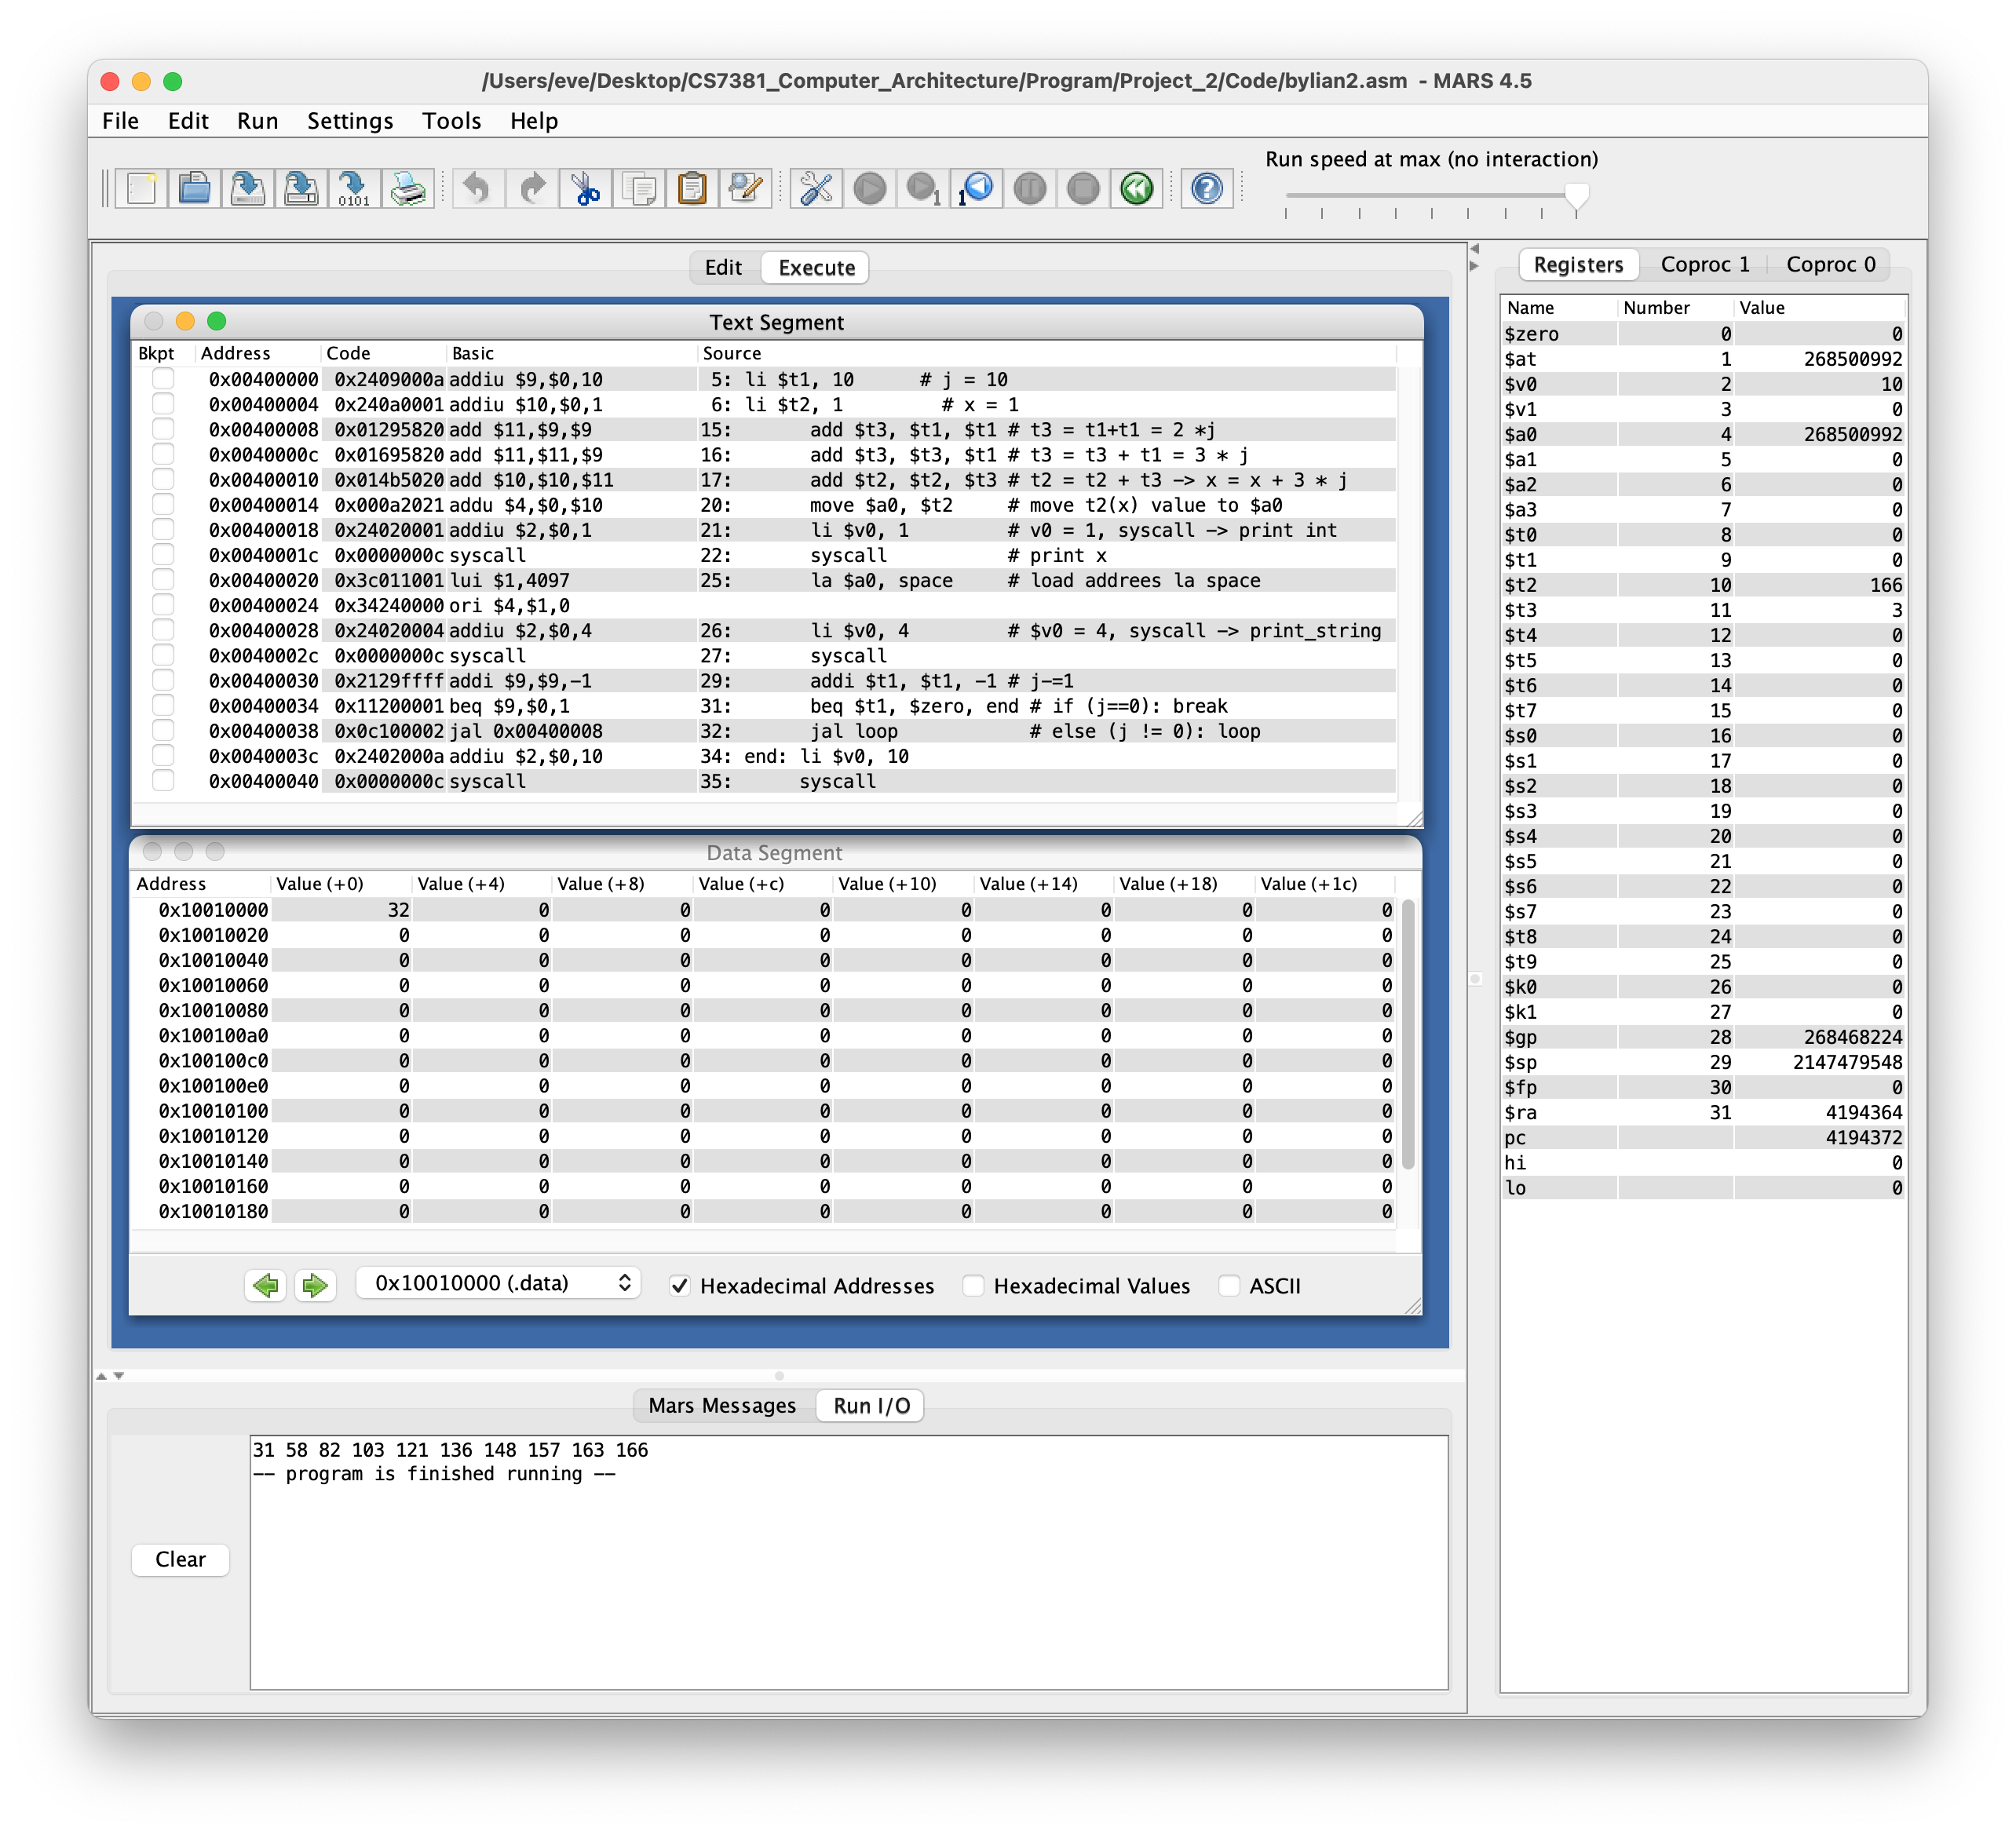
\includegraphics[width=1.1\textwidth]{p1.png} 
        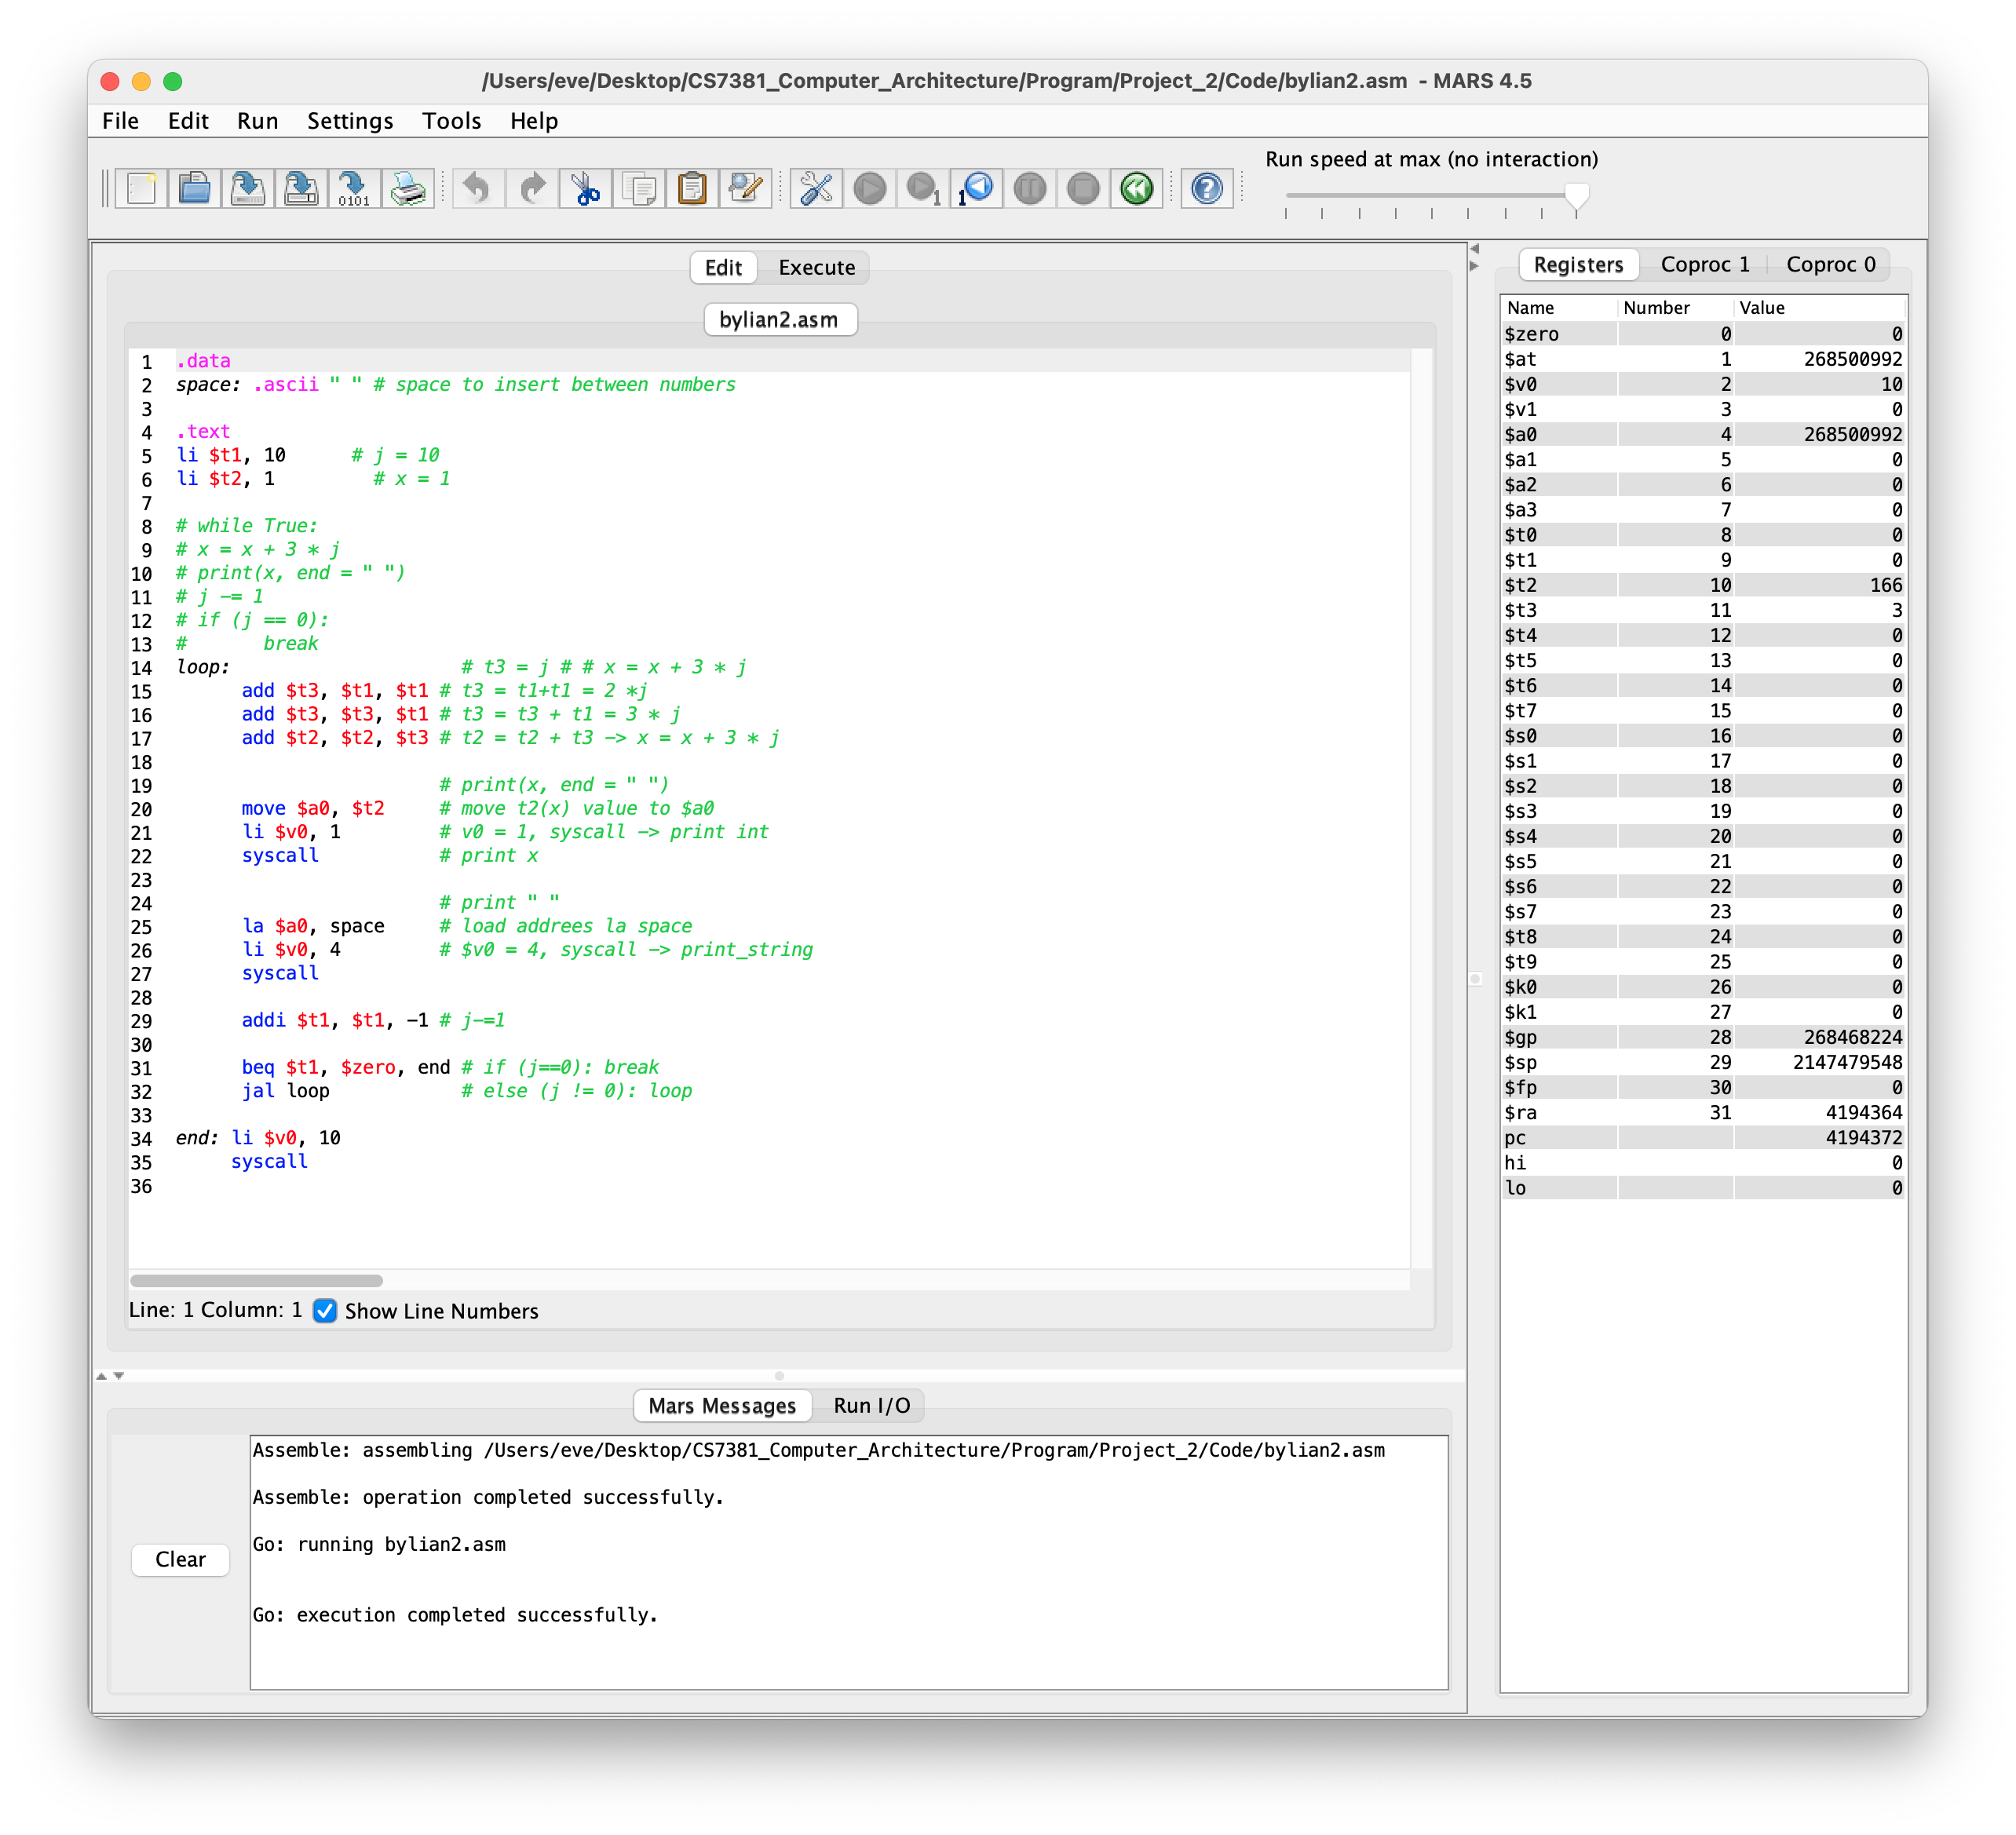
\includegraphics[width=1.1\textwidth]{p2.png}
    \end{center}

\end{document}
